
\documentclass[10pt]{article}
\usepackage[margin=1in]{geometry}
\usepackage{amsmath}
\usepackage{amssymb}
\usepackage{setspace}
\usepackage{graphicx}
\usepackage{caption}
\usepackage{listings}


\begin{document}

\title{ECE 4750 Lab 4: Ring Network}
\author{Avinash Navada (abn44) \& Akshay Dongaonkar (akd54) \& Vivek Gaddam (vrg22)}
\maketitle


\section{Introduction}

With processors hitting the power wall and Moore's Law not the primary vehicle
in increasing general computing performance, designers have chosen to
replicate processing units on a single chip. 
This process is called parallelism. 
The idea is that multiple compute units can do different work at the same time
to increase performance.
However, when multiple compute units need to communicate, they need a network
to pass their messages. \par

Given that many tasks are not easily made parallel, there is message overhead.
This leads to designers needing to develop a fast and reliable
on chip interconnect network.
In this lab, we explore the performance of a ring topology under multiple
routing algorithms. \par

In the project management section, we will lay out our project roadmap,
distribution of work, and member roles.
In the baseline design section, we will describe our ring topology and our 
greedy oblivious routing algorithm.
In the alternative design section, we will describe an updated routing 
algorithm to increase performance under adversarial traffic patterns.
In the evaluation section, we compare the performance under both routing
algorithms and the performance of the topology in general.


\section{Project Management}

We assigned Akshay to be the architect,
Avinash to be the verification lead,
and Vivek to be the design lead.
Our initial project roadmap was rather aggressive and required us to be 
finished by Sunday, November 9\textsuperscript{th}, since we planned on 
trying out an extension or two for this lab. 
Our expected and actual work patterns are shown in Figure~\ref{fig:gantt}.
Clearly, we still have not gotten the hang of working under a predictable
and incremental schedule pattern.
We aim to fix this for the final lab.
It is our last chance to do so, and we are highly motivated in this goal.
 \par

The work was divided as follows:
Vivek worked on most of the baseline RTL code.
Akshay worked exclusively on the writeup and the evaluations of the designs.
Avinash finished the baseline design and implemented the alternative design.
He also completed our testing suite.
Akshay's work was lacking in this lab; he was sick most of the first week
and part of the second week of this lab. \par

The work was approached by simultaneously starting the baseline 
implementation and testing, followed by the lab writeup shortly after.
Baseline paths that were completed were promptly tested. 
As soon as the baseline implementation was complete and successfully tested, 
Avinash moved on to the alternative design implementation and testing 
(which included adding additional test cases for the alternative design). 
Each team member helped others debug as much as they could. 
Due to Akshay being sick and Vivek having a tough workload in other classes,
we were unable to implement an extension. 
We are sad that we were unable to complete an extension even at the advanced
stage of this semester. 


\section{Baseline Design}

The baseline design for our lab network has 8 nodes in a ring configuration
for its topology. 
Each node contains a message producer/consumer (also known as Input/Output 
terminals), a router that the terminal connects to,
and two outgoing channels from the router to other routers in the ring.
Therefore, each router has three total input and output channels.
The ring is given its topology by the west channel of router $n$ connecting 
to router $n-1$ and the east channel of router $n$ connecting to router $n+1$.
The exception is that the west channel of router $0$ connects to router $7$
and the east channel of router $7$ connects to router $0$.
This topology is logicaly shown in Figure~\ref{fig:topo}. \par
% Figure reference not working... Figure it out.

The messages that our network transmit have a parametrized structure.
There is a payload size, a source/destination tag size determined by the number
of addresses (in our case eight), and an opaque bit size.

These messages are 


\section{Alternative Design}


\section{Testing Strategy}


\section{Evaluation}

\newpage

\section {Tables and Diagrams}



% % Figure: Gantt Chart

\begin{figure}[h]
\centering
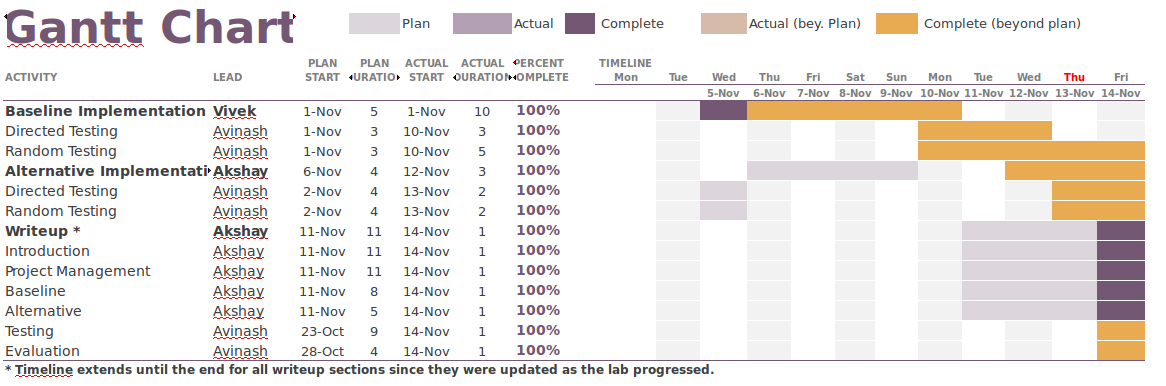
\includegraphics[scale=0.4, angle=90]{gantt}
\caption{Gantt Chart}
\label{fig:gantt}
\end{figure}

\begin{figure}
\centering
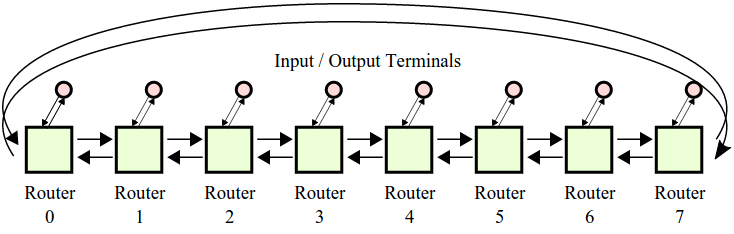
\includegraphics[scale=0.5]{topology}
\label{fig:topo}
\caption{Network Topology of our Ring}
\end{figure}


\end{document}






